\section{Aplikace a objekty}
%%%%%%%%%%%%%%%%%%%%%%%%%%%%
\subsection{Aplikace}
Aplikace slouží pro seskupení záložek a domovských stránek na jednom místě.

V systémovém nastavení, byla v menu \emph{App Manager} vytvořena nová aplikace \emph{Lava Design}. Aplikace byla vytvořena pomocí tlačítka \emph{New Lightning App}, které spouští průvodce tvorby nové aplikace s moderním uživatelským rozhraním Lightning.

Přehled základních informací o aplikaci je vidět na obrázku \ref{fig:LD_app_info}.

Aplikace je potom dostupná ze záložky pro spuštění aplikací, jak je vidět na obrázku\ref{fig:app_launcher}.
\begin{figure}[h!]
    \centering
    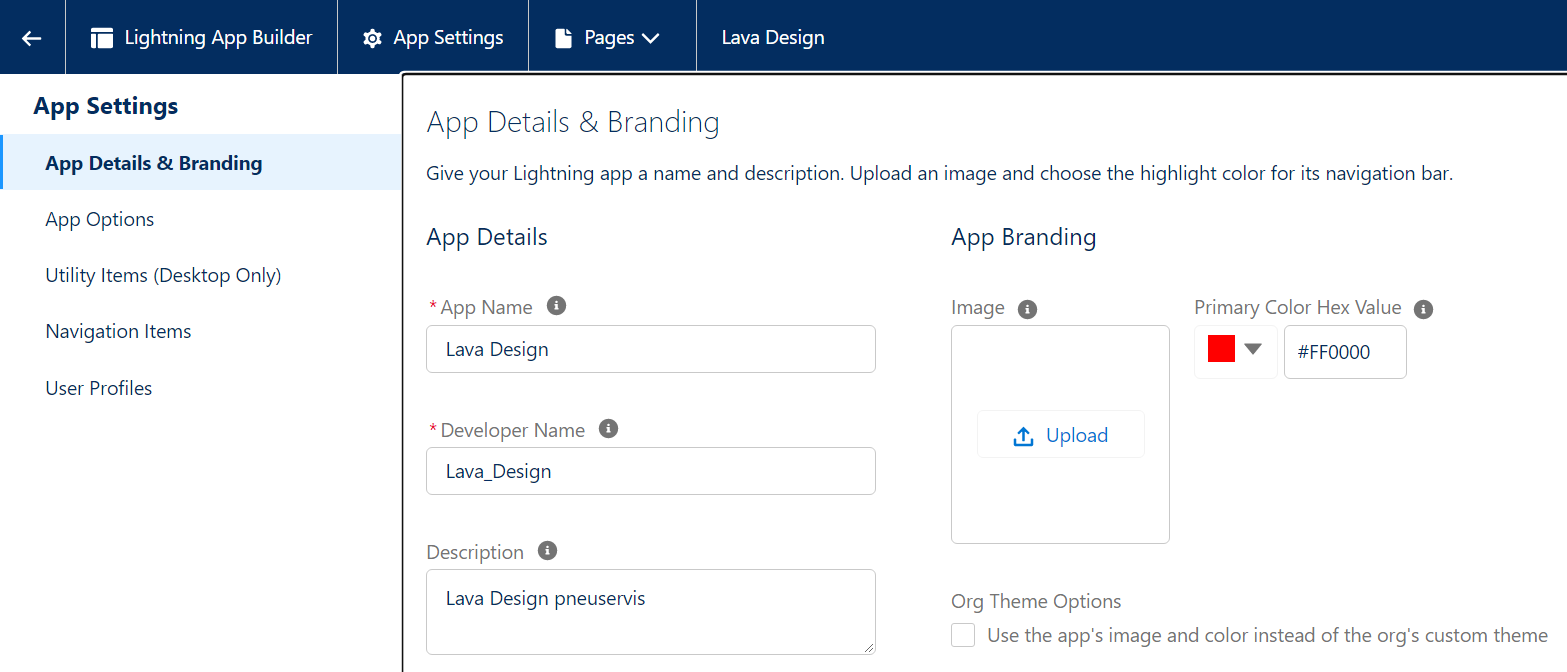
\includegraphics[width=\textwidth]{assets/7_implementace/aplikace_a_objekty/LD app.png}
    \caption{Obecné informace o aplikaci Lava Design.}
    \label{fig:LD_app_info}
\end{figure}
\begin{figure}[h!]
    \centering
    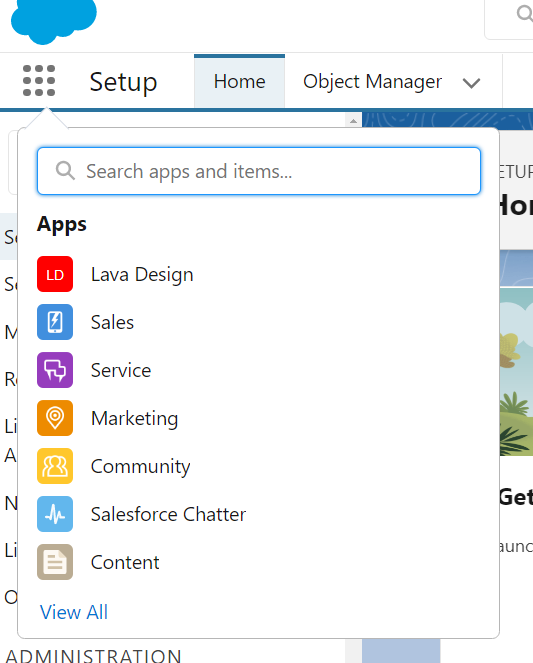
\includegraphics[width=0.4\textwidth]{assets/7_implementace/aplikace_a_objekty/app launcher.png}
    \caption{App Launcher.}
    \label{fig:app_launcher}
\end{figure}
\FloatBarrier
%%%%%%%%%%%%%%%%%%%%%%%%%%%%
\subsection{Objekty}
Entity z návrhu \ref{fig:Domain_model_-_new} byly replikovány v systému Salesforce pomocí vlastních objektů. 

Vlastní objekty jsou objekty vytvořené administrátory, těmto objektům je možné změnit jméno a atributy.

Systém Salesforce již obsahuje řadu standardních objektů. Ty se pro tuto aplikaci nehodí, protože obsahují velké množství nadbytečných atributů a již jsou zatíženy vazbami na jiné objekty. Z tohoto důvodu byly vytvořeny nové vlastní objekty. 

Tvorba objektů proběhla skrze záložku \emph{Object Manager} a \emph{Schema Builder}, který poskytuje interaktivní schéma pro tvorbu objektů a vazeb mezi nimi. 

Některým objektům byly přidány další potřebné atributy a vazby, které v původním návrhu nejsou. Oproti původnímu modelu byly přidány vazby mezi zákazníkem a službami, a to hlavně kvůli rychlejší práci v systému.

Finální schéma je vidět na obrázku \ref{fig:Object_schema_builder}.
\begin{sidewaysfigure}[h!]
    \centering
    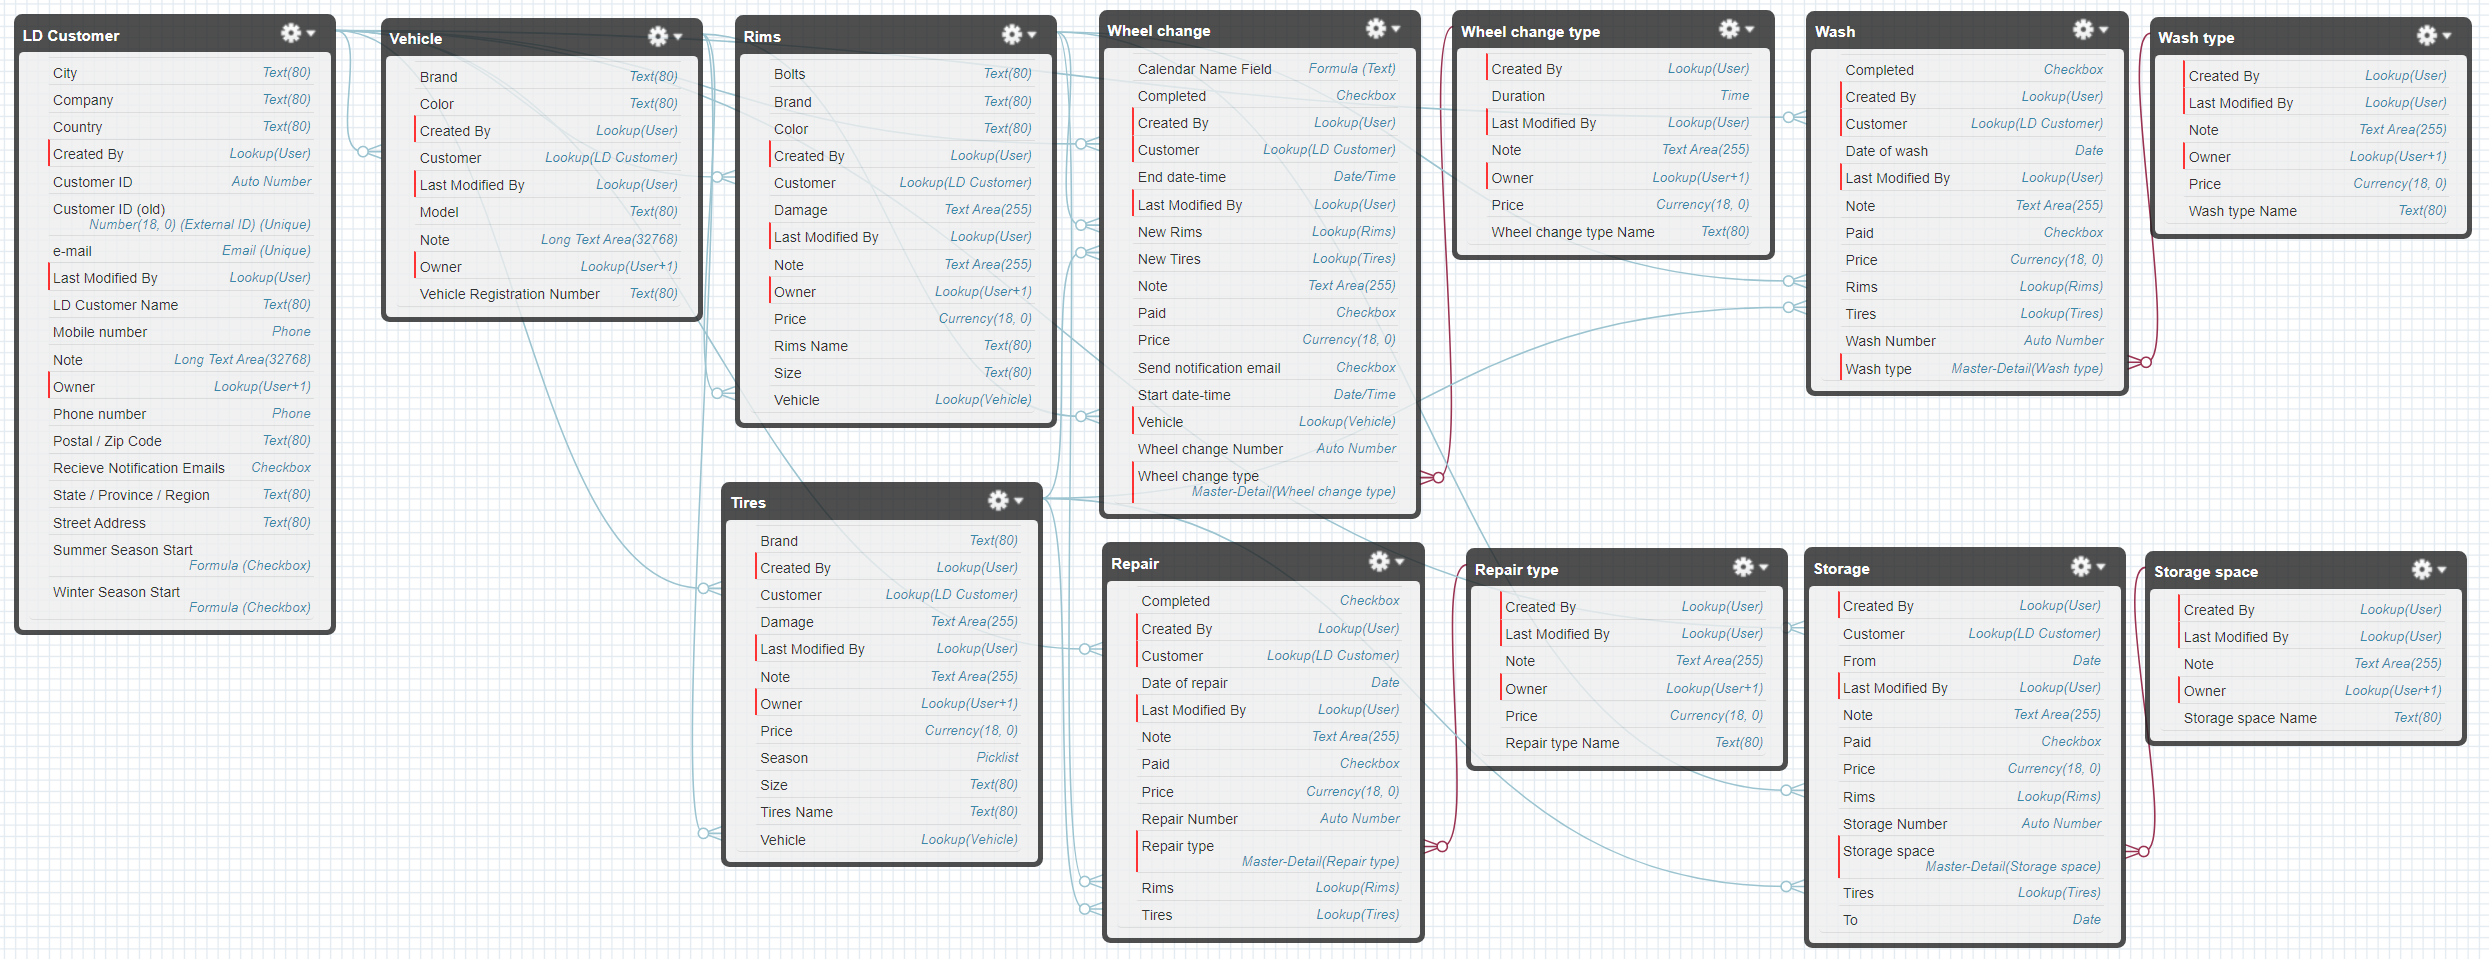
\includegraphics[width=\textwidth]{assets/7_implementace/aplikace_a_objekty/Schema builder.png}
    \caption{Schéma objektů.}
    \label{fig:Object_schema_builder}
\end{sidewaysfigure}
\FloatBarrier

Během vytváření nových objektů je třeba dbát, aby jejich názvy nekolidovaly s názvy standardních objektů v systému Salesforce. To je vidět na objektu \emph{LD Customer}, na obrázku \ref{fig:LD_customer}, který má znázorňovat zákazníka. Tento objekt byl pojmenován s předponou \emph{LD}, aby se odlišil od standardního objektu \emph{Customer}. 

\begin{figure}[h!]
    \centering
    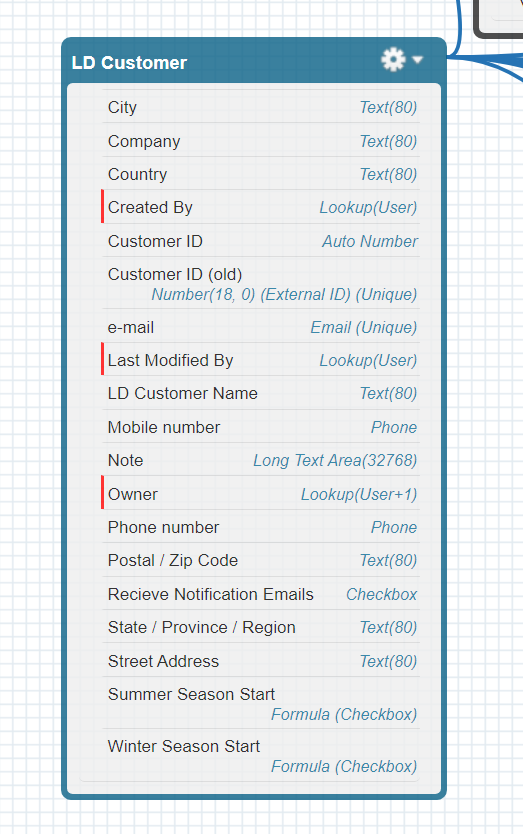
\includegraphics[width=0.45\textwidth]{assets/7_implementace/aplikace_a_objekty/LD Customer.png}
    \caption{Objekt zákazníka.}
    \label{fig:LD_customer}
\end{figure}
\FloatBarrier
%%%%%%%%%%%%%%%%%%%%%%%%%%%%
\subsection{Záložky}
Záložky slouží pro zobrazení seznamů záznámů objektů. Dříve vytvořeným objektům byly vytvořeny záložky v menu \emph{Tabs}.

V nastavení aplikace \emph{Lava Design} byly tyto záložky přidány seznamu záložek. Do záložek aplikace byly přidány i záložky \emph{Home} a \emph{Calendar}. Výsledkem jsou záložky v aplikaci, které jsou vidět na obrázku \ref{fig:LD_app_tab}.

\begin{figure}[h!]
    \centering
    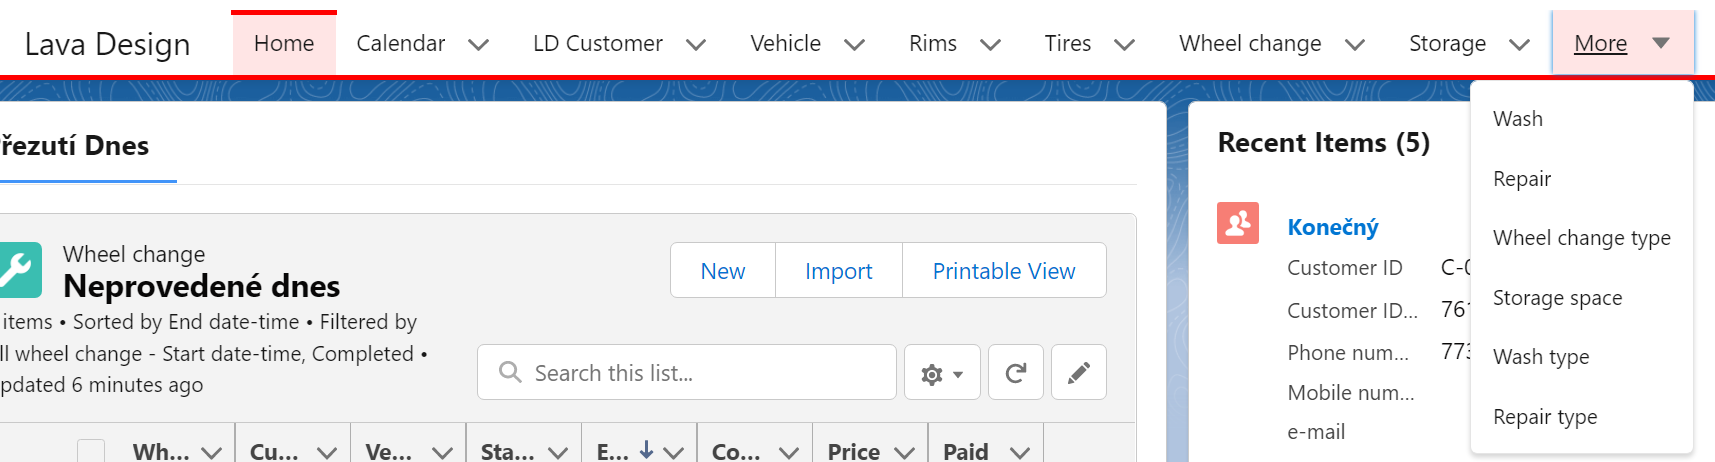
\includegraphics[width=\textwidth]{assets/7_implementace/aplikace_a_objekty/LD tabs.png}
    \caption{Záložky v aplikaci Lava Design.}
    \label{fig:LD_app_tab}
\end{figure}
\FloatBarrier
